\chapter{Implementacja} \label{chap:implementation}

\section{Opis modelu danych do reprezentacji skrzyżowań}

W opracowanym rozwiązaniu drogi reprezentowane są w sposób dyskretny. Każda droga zaczyna się w pozycji 1 i rośnie wraz z jej rozmiarem. Samochody poruszają się po drogach w następujących kierunkach:
\begin{itemize}
\item z północy na południe
\item z południa na północ
\item z zachodu na wschód
\item ze wschodu na zachód
\end{itemize}
Powyższe ogarniczenie nie wpływa na algorytm lub wyniki. Dodanie funkcjonalności wymagałoby dodania możliwości zmiany numeru drogi przez samochód, co nie wpływa na liczbę stanów, a co za tym idzie długość wykonywania algorytmu.
\newline
\newline
Droga jest reprezentowana poprzez:
\begin{itemize}
\item unikatowy numer drogi
\item rozmiar drogi
\item informacja o przecięciach z innymi drogami
\item kierunek w którym samochód się porusza na drodze (z północy na południe, czy z południa na północ lub z zachodu na wschód czy ze wschodu na zachód)
\end{itemize}
Samochody na drogach są opisane przez:
\begin{itemize}
\item unikatowy numer samochodu
\item unikatowy numer drogi, na której pojazd się znajduje
\item numer pozycji na drodze, na której samochód się znajduje
\item prędkość początkowa
\item numer pozycji docelowej na drodze - punkt za ostatnim skrzyżowaniem
\end{itemize}
Samochody poruszają się po drogach w krokach czasowych. Prędkość samochodu wyrażana jest w liczbie odcinków drogi na jeden krok czasowy.
\newline
\indent
W Systemie można wybrać maksymalne przyspieszenia ujemne oraz dodatnie samochodów z następujących możliwości \{-2, -1, 0, 1, 2\}. Oznacza to, że w następnym stanie pojazd może przyspieszyć o 1 lub 2 odcinki drogi na jeden krok czasowy. Dla wartości 0 pojazd utrzymuje swoją prędkość. Dla wartości ujemnych pojazd zwalnia o 1 lub 2 odcinki drogi na jeden kroku czasowym. Ilość możliwych dla samochodu przyspieszeń znacznie wpływa na złożoność czasową algorytmu, z tego względu, że wraz ze wzrostem ilośći możliwych przyspieszeń rośnie ilość możliwość stanów sąsiednich dla samochodu, przez które algorytm musi przejść.        
\newline
\indent
Do modelu przekazać należy także maksymalną prędkość, którą wszystkie samochody mogą osiągnąć oraz parametr prędkości, czyli liczba pozyji będąca dystansem trzymanym między pojazdami.

\section{Zmodyfikowany algorytm A*}

Zaprezentowany w tej pracy zmodyfikowanym algorytmu A* jest oparty na stanach, gdzie pojedyńczym stanem jest rozłożenie samochodów na drogach wraz z ich prędkościami. Algorytm zaczynając od zadanego stanu początkowego analizuje możliwe stany sąsiednie i wybiera optymalną ścieżkę kierując się funkcją heurystyki. Ścieżka prowadzi do określonego celu. W przypadku opracowanego rozwiązania, celem jest przekroczenie przez wszystkie samochody ostatniego skrzyżowania na drogach, na których się znajdują.
\newline
\indent
Zrealizowany Algorytm A* jest generyczny. Do algorytmu przekazujemy klasę reprezentującą dowolny stan. Klasa musi implementować metodę 'neighbours', która zwraca stany sąsiednie dla danej instancji stanu. Do algorytmu przekazywana jest także funkcja heurystyki, zależna od danych danego stanu.
\newline
\indent
Modyfikacja róźni się od innych tym, że stany sąsiednie są liczone dynamicznie. Algorytm nie ma z góry podnaego celu. Dla przykładu w przeszukiwaniu ścieżki w grafie celem jest podany wierzchołek końcowy. Algorytm przyjmuje funkcje wygranej, która określa warunki końca algorytmu. W przedstawionej pracy warunkiem końca jest przekroczenie przez wszystkie pojazdy skrzyżowań.

\section{Stan w opracowanym rozwiązaniu dla algorytmu A*}

Stan w modyfikacji algorytmu A* przedstawionej w tej pracy opisuje stan wszystkich samochodów na skrzyżowaniach wraz z ich prędkościami. Zgodnie z wcześniej opisaną generycznością wierzchołek jest obiektem klasy, który implementuje metodę 'neighbours'. Metoda generuje wszystkie stany sąsiednie dla aktualnego stanu. Dla przykładu, dla ustawień przyspieszeń \{-2, -1, 0, 1, 2\}, dla każdego z aut na skrzyżowaniu generowane są stany z jego prędkością dodając wartości przyspieszeń. Pomijane są stany, w których prędkość samochodu byłaby ujemna. Przykładowo jest pojazd z prędkością 1 pozycji na krok czasowy znajdujący się na 1 pozycji na drodze numer 1. Dla pojazdu rozpatrywane są następujące stany:
\begin{enumerate}
\item Dodając przyspieszenie o wartości 0: 2 pozycja na drodze numer jeden z prędkością 1
\item Dodając przyspieszenie o wartości 1: 3 pozycja na drodze numer jeden z prędkością 2
\item Dodając przyspieszenie o wartości 2: 4 pozycja na drodze numer jeden z prędkością 3
\item Dodając przyspieszenie o wartości -1: 1 pozycja na drodze numer jeden z prędkością 0
\item Dodając przyspieszenie o wartości -2: Stan jest eliminowany, ponieważ prędkość byłaby ujemna
\end{enumerate}
Dodatkowo w przypadku ustawienia maksymalnej prędkości równej 2 pozycje na jeden krok czasowy - możliwość nr 3 także zostałaby wyeliminowana.
\newline
\newline
W metodzie usuwane są także stany powodujące kolizje, co będzie opisane w następnym rozdziale.

\section{Unikanie kolizji}

Koniecznym elementem w koordynacji ruchu na skrzyżowaniach wielu pojazdów jest unikanie kolizji. W opracowanym rozwiązaniu nikanie kolizji zostało podzielone na dwa etapy:
\begin{enumerate}
\item Unikanie kolizji aut poruszających się po tym samym pasie
\item Unikanie kolizji na skrzyżowaniach
\end{enumerate}
Implementacja unikania kolizji pojazdów na tym samym pasie polega na policzeniu obszarów dla samochodów znajdujących się na tym samym pasie, który będą one obejmowały w jednym kroku czasowym wraz z uwzględnieniem parametru bezpieczeństwa. Jeżeli obszary dwóch samochdów na jednym pasie pokrywają się - taki stan jest usuwany i wówczas metoda 'neighbours' nie zwróci go jako stanu sąsiedniego. Na rysunku \ref{collision-avoidance-lane} przedstawiony jest przykład unikania kolizji dla samochodów poruszających się jednym pasem. Przykład przedstawiony jest z parametrem bezpieczeństwa równym jeden. Samochody, mając przed sobą inny pojazd, czekają aż będzie dla nich miejsce.
\begin{figure}
    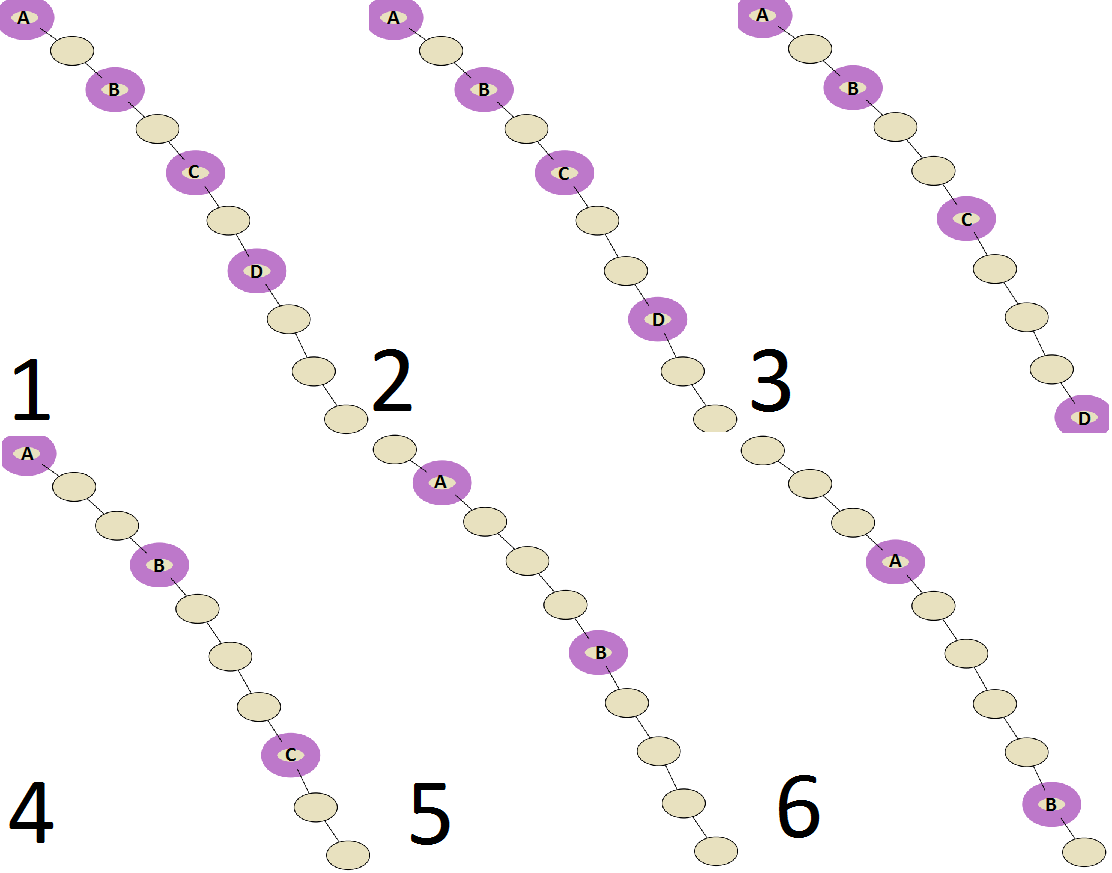
\includegraphics[width=1.0\textwidth]{collision-avoidance-lane.png}
  \caption{Unikani kolizji na pasie}
  \label{collision-avoidance-lane}
\end{figure}
\newpage
Unikanie kolizji na skrzyżowaniach polega na eliminacji stanów, w których conajmniej dwa auta przekroczyły w jednym kroku czasowym to samo skrzyżowanie. Metoda 'neighbours' także nie zwróci takich stanów. Na rysunku \ref{collision-avoidance-crossroads} przedstawiony jest przykład unikania kolizji dla dwóch samochodów na prostym skrzyżowaniu. Samochód z numerem jeden przyspieszył o dwie jedostki i zmienił pozycję o dwie jednostki do przodu. Samochód z numerem dwa przyspieszył natomiast o jedną jednostkę i zmienił pozycję o jedną jednostkę do przodu w celu uniknięcia kolizji. W algorytmie usunięty został stan, w którym oba pojazdy przyspieszyły o dwie jednostki. Został natomiast wybrany stan gdzie jeden z samochodów przyspieszył o dwie jednostki, a drugi o jedną jednostką, ponieważ prowadzi to, do najszybszego opuszczenia skrzyżowania przez pojazdy.
\begin{figure}
    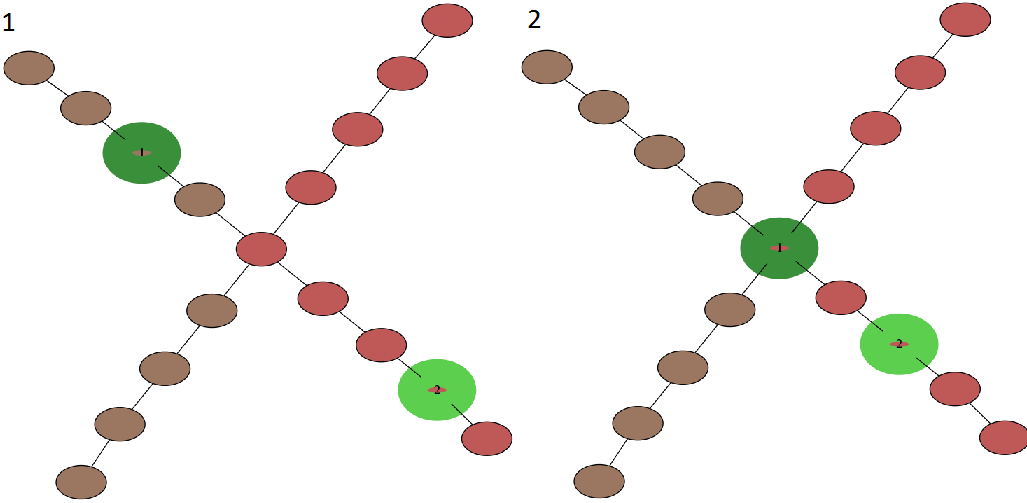
\includegraphics[width=1.0\textwidth]{collision-avoidance-crossroads.png}
  \caption{Unikanie kolizji na skrzyżowaniu}
  \label{collision-avoidance-crossroads}
\end{figure}
\newpage

\section{Format danych wejściowych}

Zaprezentowane rozwiązanie potrzebuje dane na temat skrzyżowań, samochodów oraz ograniczeń parametrów samochodów. Skrzyżowania reprezentowane są w pliku CSV posiadającym atrybuty: numer drogi, rozmiar, przecięcia, kierunek. Przecięcie reprezentowane są przez dwie liczby. Na przykład 5 7 - oznacza, że droga przecina drogę o numerze 5 w pozycji 7. Kolejne przecięcia oddzielane są średnikami. Stany samochodów zapisane są w pliku CSV posiadającym atrybuty: numer samochodu, numer drogi samochodu, pozycję na drodze, pozycję końcową. Ograniczenia przechowywane są w osobnym pliku CSV posiadającym atrybuty: maksymalna prędkość, parametr bezpieczeńśtwa, wartości przyspieszeń.

\section{Funkcja heurystyki}

Funkcja heurystyki dla algorytmu A* jest to suma kroków czasowych, po których wszystkie auta przekroczą ostatnie skrzyżowanie - czyli osiągną cel. Funkcja liczona jest, przy założeniu, że wszystkie samochody maksymalnie przyspieszają.
\newline
\indent
W opracowanym rozwiązaniu każdy samochód ma wyznaczoną pozycję, na której musi się znaleźć lub ją przekroczyć (jest to pozycja za ostatnim skrzyżowaniem). Poniżej przedstawiony jest przykład liczonej funkcji heurystyki dla dwóch stanów opisujących położenia samochodów na skrzyżowaniu.
\newline
\newline
\begin{table}[t]
    \begin{tabular}{|c|c|c|c|c|}
      \hline 
      Numer pojazdu & Numer drogi & Pozycja na drodze & Prędkość & Pozycja końcowa\\
      \hline
      1 & 1 & 1 & 1 & 6 \\
      \hline
      2 & 2 & 1 & 1 & 6 \\
      \hline
      3 & 3 & 1 & 1 & 6 \\
      \hline
      4 & 4 & 1 & 1 & 6 \\
      \hline
    \end{tabular} 
    \caption{Stan 1}
    \label{FirstState}
\end{table}
\newline
\begin{table}[t]
    \begin{tabular}{|c|c|c|c|c|}
      \hline 
      Numer pojazdu & Numer drogi & Pozycja na drodze & Prędkość & Pozycja końcowa\\
      \hline
      1 & 1 & 1 & 0 & 6 \\
      \hline
      2 & 2 & 1 & 1 & 6 \\
      \hline
      3 & 3 & 1 & 0 & 6 \\
      \hline
      4 & 4 & 1 & 1 & 6 \\
      \hline
    \end{tabular} 
    \caption{Stan 2}
    \label{SecondState}
\end{table}
\newpage
Dla stanu opisanego w tabeli \ref{FirstState} funkcja heurystyki jest liczona następująco:
\newline
\newline
\textbf{Dla pojazdów 1-4:}
\newline
\newline
\underline{1 krok czasowy}:
\newline
\newline
prędkość = (prędkość) 1 + (maksymalne przyspieszenie) 1 = 2
\newline
pozycja = (pozycja) 1 + (prędkość) 2 = 3
\newline
\newline
Pojazd znajduje się na pozycji 3, która jest przed pozycją końcową 6 - liczony jest kolejny krok czasowy.
\newline
\newline
\underline{2 krok czasowy}:
\newline
\newline
prędkość = (prędkość) 2 + (maksymalne przyspieszenie) 1 = 3
\newline
pozycja = (pozycja) 3 + (prędkość) 3 = 6
\newline
\newline
Pojazd znajduje się na pozycji 6, która jest równa pozycji końcowej.
\newline
\newline
Razem 2 kroki czasowe dla jednego pojazdu. Dla wszystkich czterech pojazdów - 8 kroków czasowych.
\newline
\newline
\newline
Dla stanu opisanego w tabeli \ref{SecondState} funkcja heurystyki jest liczona następująco:
\newline
\newline
\textbf{Dla pojazdów 1 i 3}
\newline
\newline
\underline{1 krok czasowy}:
\newline
\newline
prędkość = (prędkość) 0 + (maksymalne przyspieszenie) 1 = 1
\newline
pozycja = (pozycja) 1 + (prędkość) 1 = 2
\newline
\newline
Pojazd znajduje się na pozycji 2, która jest przed pozycją końcową 6 - liczony jest kolejny krok czasowy.
\newline
\newline
\underline{2 krok czasowy}:
\newline
\newline
prędkość = (prędkość) 1 + (maksymalne przyspieszenie) 1 = 2
\newline
pozycja = (pozycja) 2 + (prędkość) 2 = 4
\newline
\newline
Pojazd znajduje się na pozycji 4, która jest przed pozycją końcową 6 - liczony jest kolejny krok czasowy.
\newline
\newline
\underline{3 krok czasowy}:
\newline
\newline
prędkość = (prędkość) 2 + (maksymalne przyspieszenie) 1 = 3
\newline
pozycja = (pozycja) 4 + (prędkość) 3 = 7
\newline
\newline
Pojazd znajduje się na pozycji 7, która jest za pozycją końcową 6.
\newline
\newline
Razem 3 kroki czasowe dla jednego pojazdu. Dla pojazdów 1 i 3 - 6 kroków czasowych.
\newline
\newline
\textbf{Dla pojazdów 2 i 4:}
\newline
\newline
\underline{1 krok czasowy}:
\newline
\newline
prędkość = (prędkość) 1 + (maksymalne przyspieszenie) 1 = 2
\newline
pozycja = (pozycja) 1 + (prędkość) 2 = 3
\newline
\newline
Pojazd znajduje się na pozycji 3, która jest przed pozycją końcową 6 - liczony jest kolejny krok czasowy.
\newline
\newline
\underline{2 krok czasowy}:
\newline
\newline
prędkość = (prędkość) 2 + (maksymalne przyspieszenie) 1 = 3
\newline
pozycja = (pozycja) 3 + (prędkość) 3 = 6
\newline
\newline
Pojazd znajduje się na pozycji 6, która jest równa pozycji końcowej.
\newline
\newline
Razem 2 kroki czasowe dla jednego pojazdu. Dla pojazdów 2 i 4 - 4 kroki czasowe.
\newline
\newline
Razem dla wszystkich pojazdów - 10 kroków czasowych.
\newline
\newline
\newline
Podsumowując, dla stanu opisanego w tabeli \ref{FirstState} funkcja heurystyki zwróci wartość 8 (osiem kroków czasowych), a dla stanu opisanego w tabeli \ref{SecondState} funkcja heurystyki zwróci wartość 10 (dziesięć kroków czasowych). Algorytm wybierze wartość minimalną - czyli wybierze stan opisany w tabeli \ref{FirstState}.

\section{Reprezentacja graficzna wyników}

W celu graficznej reprezentacji wyników zaimplementowany został moduł graficzny. Działanie modułu graficznego oparte jest na rysowaniu grafów z wykorzystaniem biblioteki Graphviz oraz jej implementacji w języku Ruby. Skrzyżowanie jest reprezentowane za pomocą grafu. Wierzchołkami grafu są poszczególne odcinki dróg. Krawędziami grafu są połączenia pomiędzy odcinkami. Samochody poruszające się po tej samej drodze są zaznaczone grubszym obwodem oraz mają ten sam kolor. Samochody można rozróżnić poprzez unikatowy numer na nich napisany. Kolejne kroki czasowe reprezentowane są poprzez następne grafy z kolejnymi ułożeniami samochodów. Efektem końcowym jest stworzony GIF z następujących po sobie grafów przy użyciu biblioteki 'rmagick' dla języka Ruby.
\newline
\indent
Moduł graficzny wczytuje wszystkie dane wejściowe: pozycję samochodów, dane skrzyżowania oraz ograniczenia. Kolejno na wejście otrzymuje plik zawierający JSON, który reprezentuje wszystkie stany samochodów na skrzyżowaniach od momentu startu, aż do opuszczenia skrzyżowań przez wszystkie samochody. Plik powstaje w wyniku wykonania zaprezentowanego algorytmu A*. Moduł wczytując dane początkowe tworzy graf bazowy. Graf bazowy przedstawia skrzyżowanie wraz z pojazdami. Kolory dla dróg oraz samochodów są losowane oraz przetrzymywane w zbiorze tak, aby żaden z kolorów się nie powtórzył. Następnie moduł, posiadający kolejne stany w kolejnych krokach czasowych, korzysta z grafu bazowego i zmienia pozycję samochodów. Po każdym kroku czasowym zapisywane jest zdjęcie grafu z numerem kroku czasowego.
\newline
\indent
W module znajduje się także dodatkowe sprawdzanie kolizji. Jeżeli kolizja wystąpi, w danym kroku czasowym na zdjęciu dodany zostanie napis "Collision". Dzięki temu można zobaczyć prawdopodobieństwo kolizji w przypadku, gdy jeden z pojazdów nie zastosuje się do planu.
\newline
\indent
Na rysunku \ref{graphical-framework} zaprezentowane jest działanie modułu graficznego dla skrzyżowania czterech dróg i ośmiu pojazdów. Na 11 elemencie rysunku widać, że wszystkie samochody opuściły wszystkie skrzyżowania po 11 krokach czasowych.
\begin{figure}
    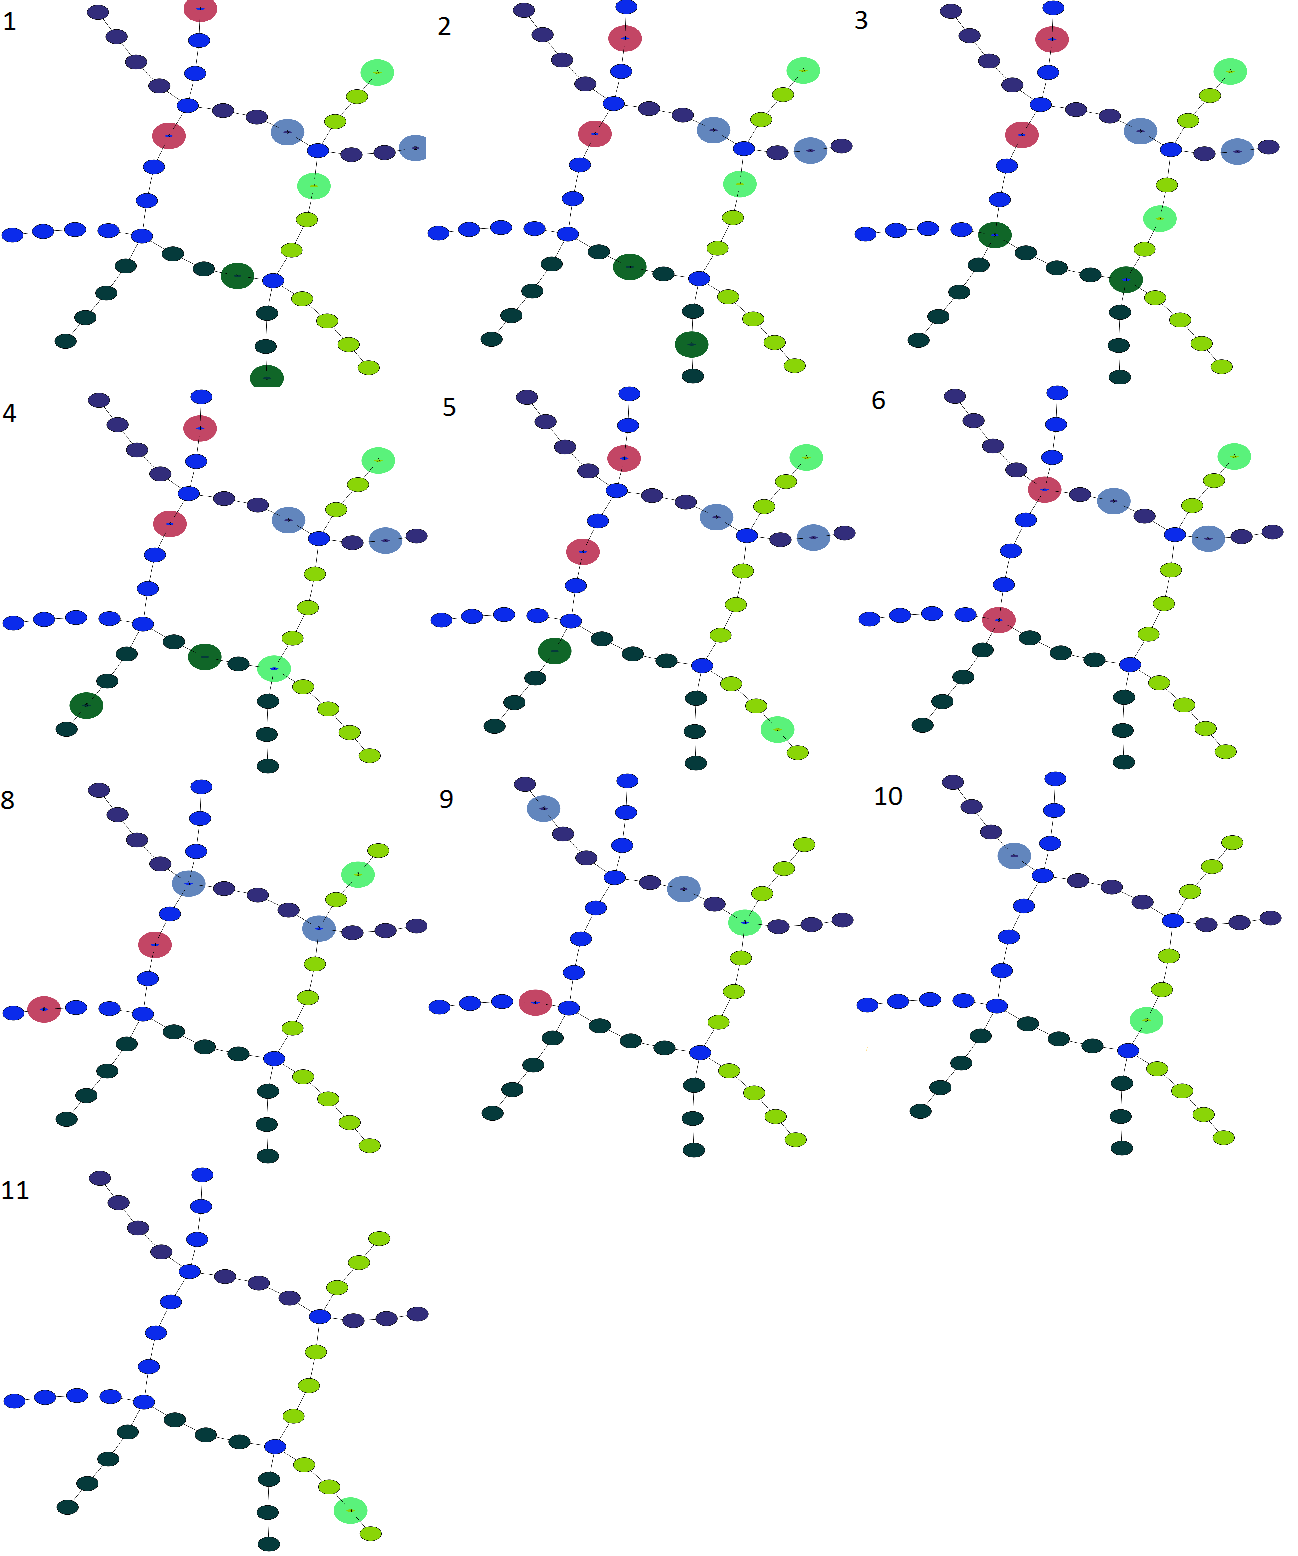
\includegraphics[width=1.0\textwidth]{graphical_module_1.png}
  \caption{Moduł graficzny}
  \label{graphical-framework}
\end{figure}
\newpage
